\chapter{Compréhension et Préparation des Données}

\section{Collecte de données}
Pour ce projet, nous avons utilisé un dataset public disponible sur Kaggle, spécialement conçu pour la détection des textes générés par intelligence artificielle. Ce dataset contient deux colonnes : la colonne text, qui contient le texte à analyser, et la colonne generated, qui sert de label indiquant si le texte a été écrit par un humain (0) ou généré par une IA (1).
\\
\begin{figure}[h!]
    \centering
    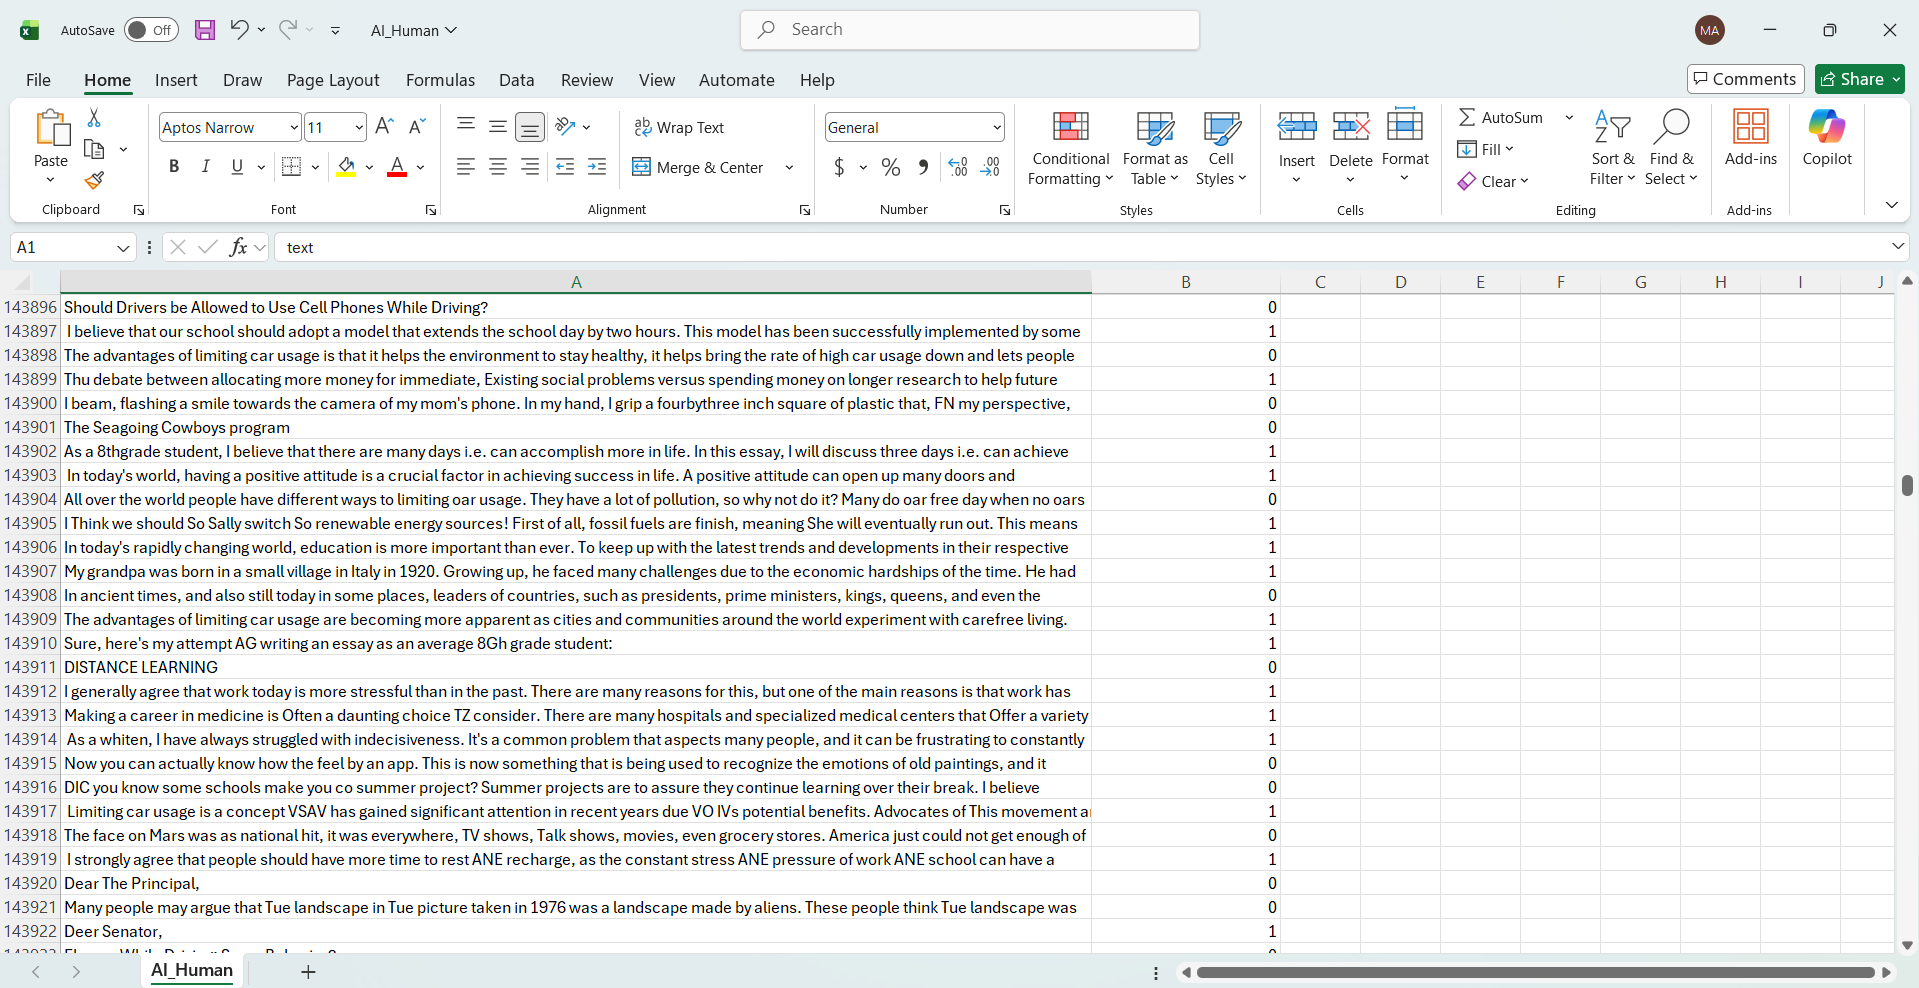
\includegraphics[width=1\textwidth]{2026.png}
    \caption{Dataset pour la détection des textes IA vs humains.}
    \label{fig:conf_matrix}
\end{figure}
\section{Description des données}
\subsection{Informations sur le Donneés}
L'image présente un aperçu de la structure et des caractéristiques d'un DataFrame contenant un total de 487 235 entrées.
\\
\begin{figure}[h!]
    \centering
    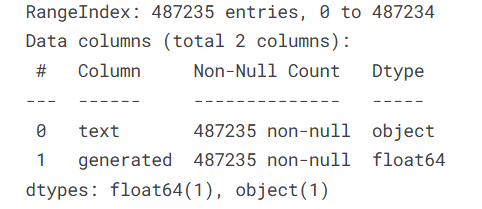
\includegraphics[width=0.6\textwidth]{Screenshot 2026-02-22 220823.png}
    \caption{Informations sur le Dataset.}
    \label{fig:conf_matrix}
\end{figure}
\\
\\
Le jeu de données est composé de deux colonnes :
\\
\\
text : Cette colonne est de type object, Elle contient 487 235 valeurs non nulles, ce qui indique qu'aucune donnée textuelle n'est manquante dans cette colonne. Il s'agit du contenu textuel à analyser.
\\
\\
generated : Cette colonne est de type float64 et contient 487 235 valeurs non nulles, confirmant l'absence de données manquantes. Comme l'indique son nom, cette variable correspond à l'étiquette binaire de classification : elle prend la valeur 1 pour les textes générés par une intelligence artificielle, et 0 pour les textes rédigés par un humain.

\subsection{Analyse statistique}
\begin{figure}[h!]
    \centering
    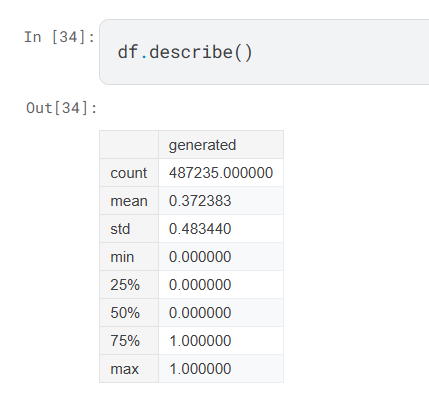
\includegraphics[width=0.4\textwidth]{Screenshot 2026-02-22 222525.png}
    \caption{Analyse statistique de la variable \texttt{generated}}
    \label{fig:conf_matrix}
\end{figure}

La fonction \texttt{df.describe()} appliquée à la variable \texttt{generated} donne les résultats suivants :
\\
\begin{itemize}
\renewcommand{\labelitemi}{-}

\item \textbf{Count = 487\,235} :  
Le dataset contient 487\,235 textes au total.

\item \textbf{Mean = 0.372} :  
Comme \texttt{generated} est une variable binaire (0 = humain, 1 = IA), cela signifie que 37,2\% des textes sont générés par une IA, tandis que 62,8\% sont écrits par des humains.

\item \textbf{Std = 0.483} :  
L'écart-type proche de 0.5 est normal pour une variable binaire modérément équilibrée.

\item \textbf{Min = 0 \quad / \quad Max = 1} :  
La variable ne contient que deux valeurs (0 et 1), ce qui confirme qu'il s'agit d'une classification binaire.

\item \textbf{25\% = 0 \quad / \quad 50\% = 0 \quad / \quad 75\% = 1} :  
La médiane égale à 0 indique que plus de la moitié des textes sont humains.  
Le troisième quartile égal à 1 montre qu'à partir de 75\% des observations, on inclut les textes générés par IA.
\\
La répartition des classes est illustrée par la courbe de distribution ci-dessous :

\end{itemize}
\begin{figure}[h!]
    \centering
    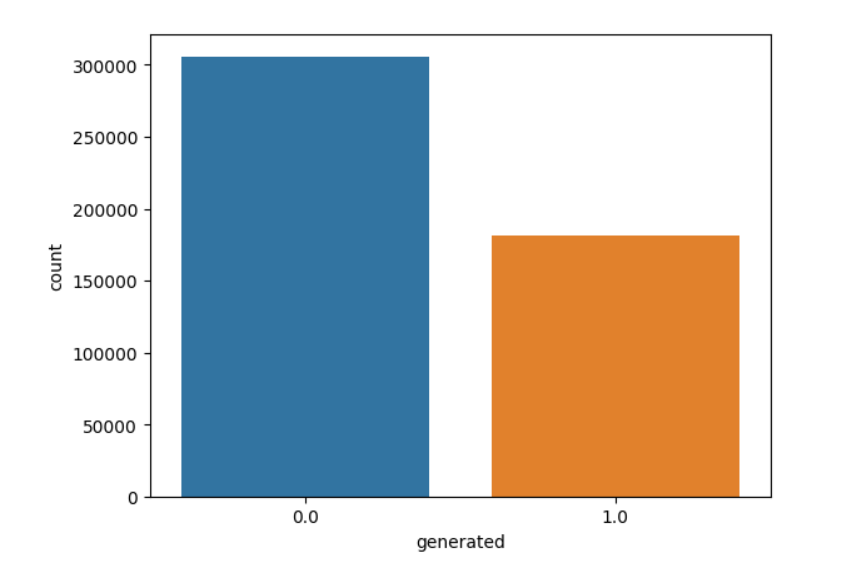
\includegraphics[width=0.8\textwidth]{Screenshot 2026-02-22 225028.png}
    \caption{Distribution des classes de la variable cible generated}
    \label{fig:conf_matrix}
\end{figure}
\section{Exploration des données}
Suite à l'observation d'un déséquilibre entre les deux classes lors de l'analyse exploratoire, une étape de rééquilibrage a été effectuée afin de garantir des conditions d'apprentissage optimales pour le modèle de classification. Pour ce faire, nous avons procédé à un sous-échantillonnage aléatoire consistant à sélectionner 50 000 échantillons de la classe majoritaire (textes humains, generated = 0) et 50 000 échantillons de la classe minoritaire (textes IA, generated = 1). 
\\
\\
Ce rééquilibrage présente plusieurs avantages :

\begin{itemize}
    \item Il élimine le biais potentiel du modèle vers la classe majoritaire.
    \item Il permet d'évaluer les performances de manière équitable sur les deux classes.
    \item Il facilite l'interprétation des métriques comme la précision et le rappel.
\end{itemize}
\\
\\
\begin{figure}[h!]
    \centering
    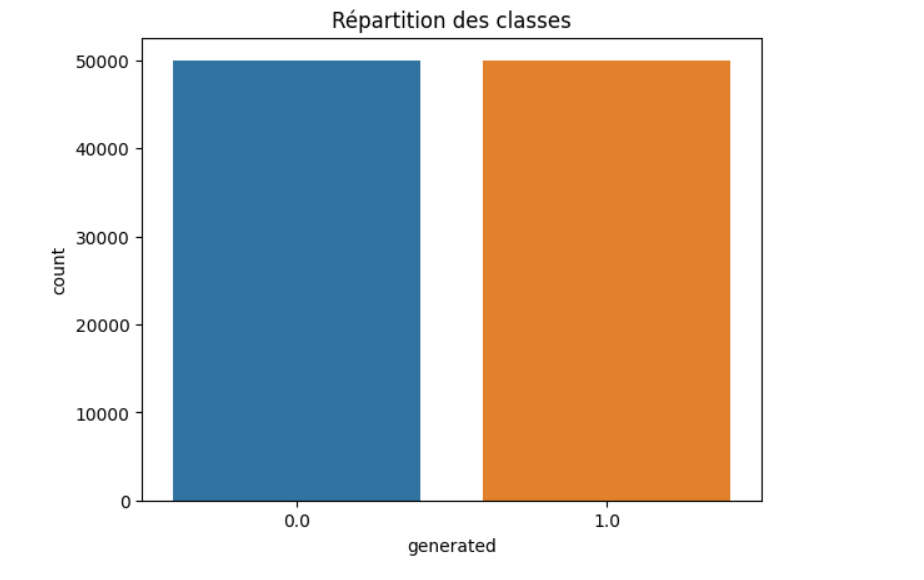
\includegraphics[width=0.8\textwidth]{2027.png}
    \caption{Distribution des classes de la variable cible generated aprés le sous-échantillonnage}
    \label{fig:conf_matrix}
\end{figure}
\\
\\

Avant d'entraîner le modèle, les textes doivent être transformés en une forme numérique compréhensible par le modèle.
Cette étape s'appelle la tokenization.
La tokenization consiste à découper un texte en petites unités appelées tokens.
Un token peut être :
• un mot complet
\\
• une partie de mot
\\
• un symbole ou un signe de ponctuation
\\  
\begin{figure}[h!]
    \centering
    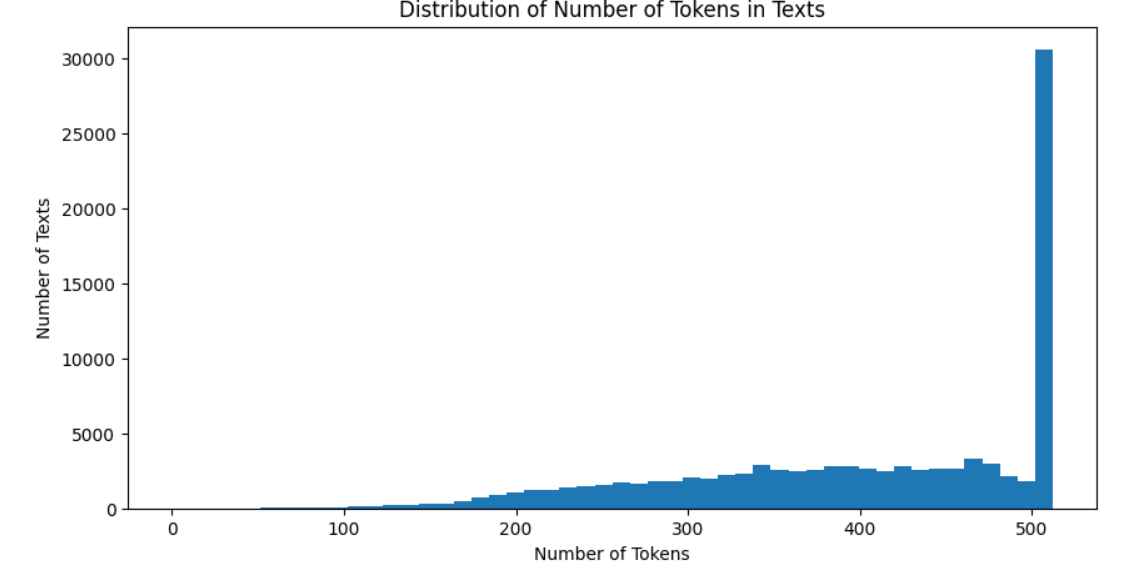
\includegraphics[width=0.8\textwidth]{2028.png}
    \caption{Distribution du nombre de tokens dans les textes}
    \label{fig:conf_matrix}
\end{figure}
\\
Ce graphique montre la distribution du nombre de tokens par texte après la tokenization.
Le pic important observé à 512 tokens indique que beaucoup de textes atteignent la limite maximale. Cela signifie que Une grande partie des textes sont longs.

\begin{figure}[h!]
    \centering
    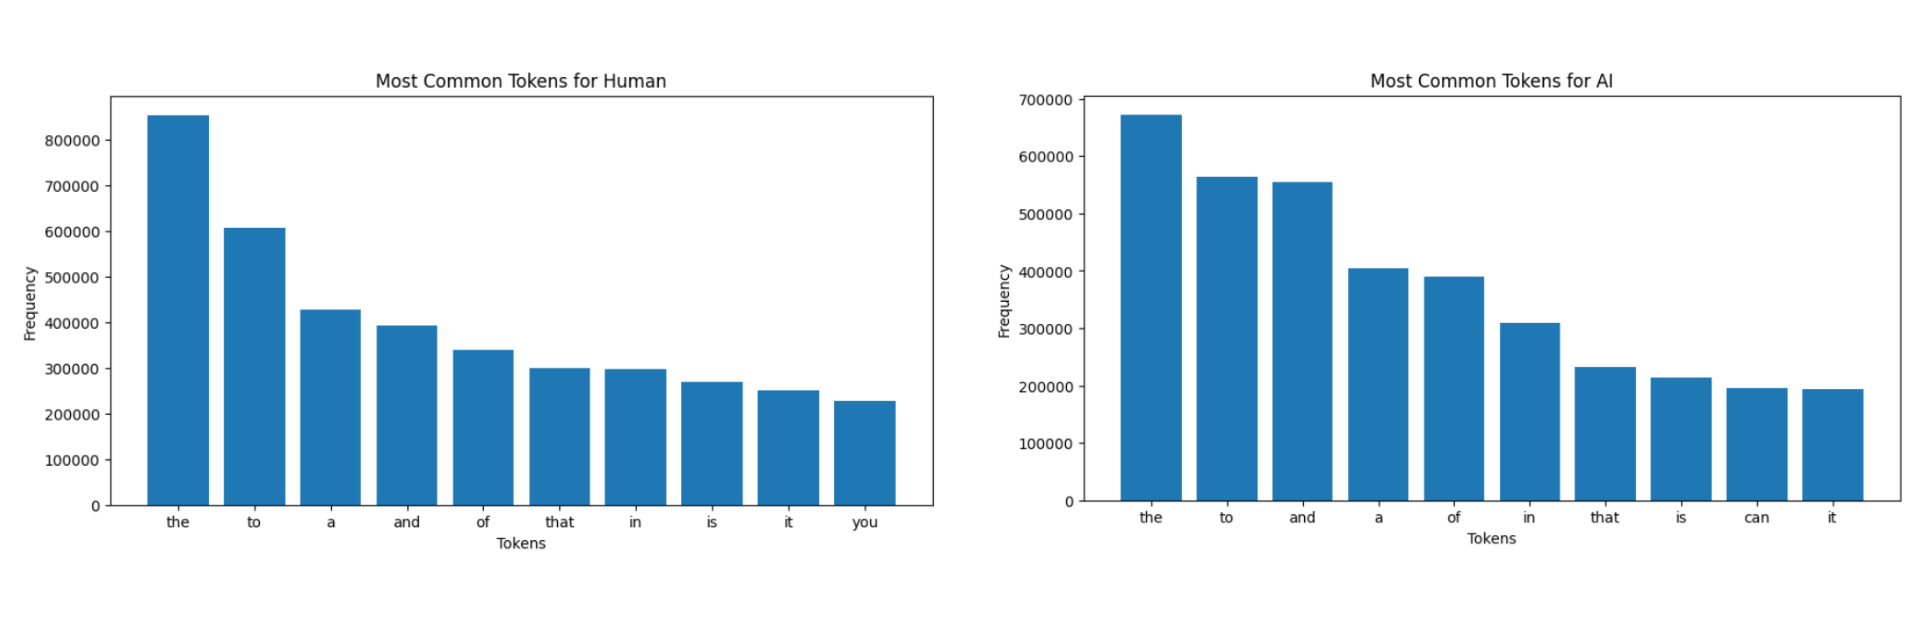
\includegraphics[width=1\textwidth]{2030.png}
    \caption{Comparaison des tokens les plus fréquents pour les textes humains et IA}
    \label{fig:conf_matrix}
\end{figure}
\\
Les graphiques présentent les tokens (mots) les plus fréquents pour les textes écrits par des humains et ceux générés par une IA.
\\
On observe que :

• Les mots les plus fréquents sont quasiment identiques dans les deux classes.

• Il s’agit principalement de mots très courants en anglais comme the, to, and, a, of, in, that, is, etc.

• Les fréquences sont également relativement similaires entre les deux catégories.
\\
\\
L’analyse des mots individuels les plus fréquents ne permet pas de discriminer efficacement les textes humains des textes générés par IA, car les distributions sont très similaires.

\begin{figure}[h!]
    \centering
    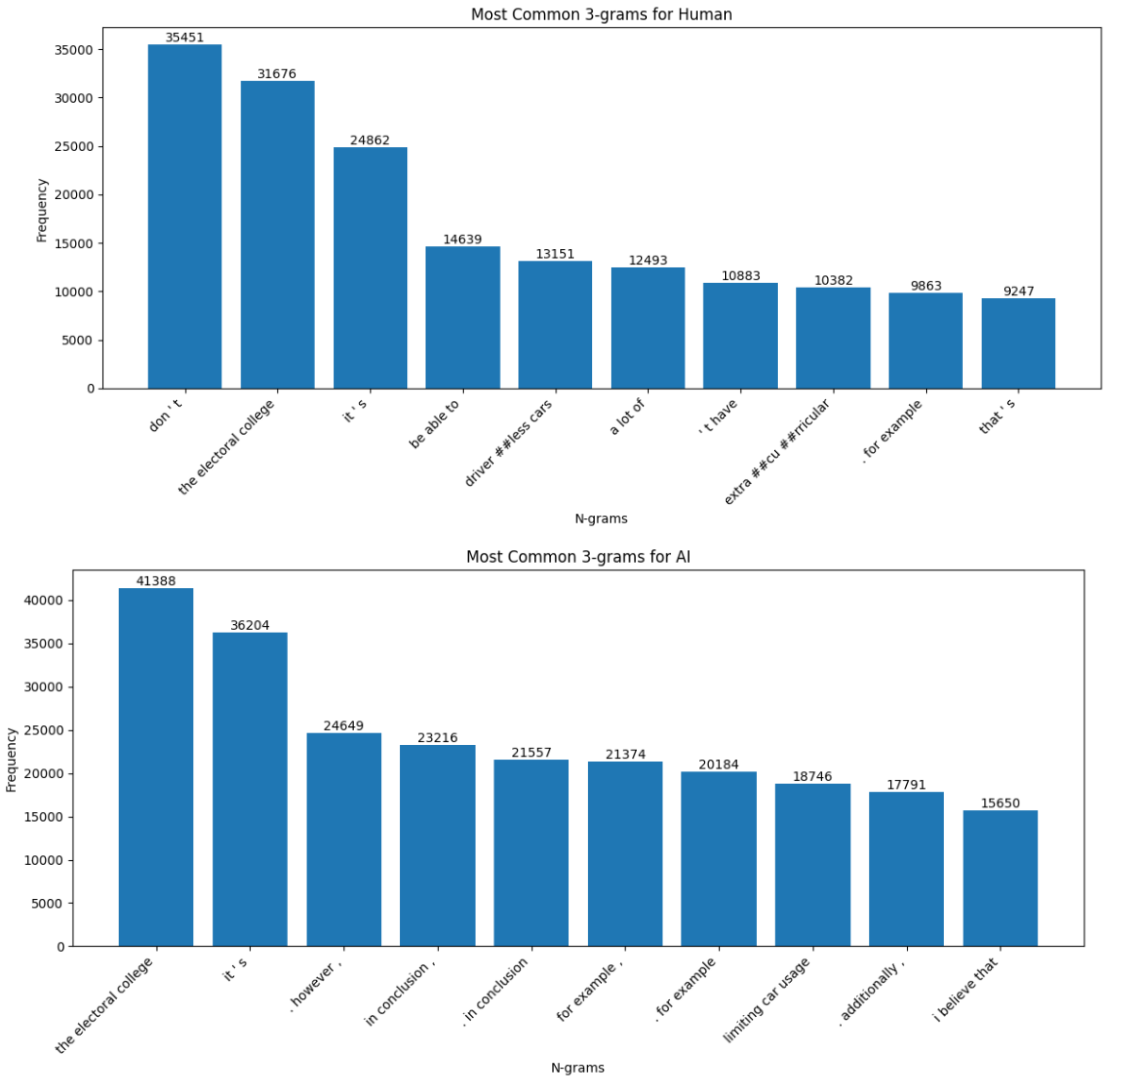
\includegraphics[width=0.7\textwidth]{777.png}
    \caption{Comparaison des 3-gramms les plus fréquents pour les textes humains et IA}
    \label{fig:conf_matrix}
\end{figure}
\\
Les graphiques présentent les 3-grams (groupes de trois mots) les plus fréquents pour les textes écrits par des humains et ceux générés par une IA.

On observe que :

• Les deux classes partagent plusieurs expressions communes, car elles traitent du même thème.

• Les textes humains utilisent davantage de tournures naturelles et conversationnelles, tandis que les textes IA emploient plus de connecteurs logiques formels et une structure plus académique.

• Lorsque l’on augmente la longueur des n-grams, les différences structurelles deviennent plus visibles et la distinction entre les deux classes s’améliore.

mais : 

• Les n-grams restent des caractéristiques purement syntaxiques et ne capturent pas la sémantique du texte.

• Les mots fréquents sont souvent communs aux deux classes, donc peu discriminants.

• Construire un modèle uniquement sur les n-grams peut conduire au surapprentissage.

Même si avoir un vocabulaire plus large aide à différencier les classes, ce n’est pas suffisant. Il faut utiliser des modèles de machine learning, comme le deep learning, pour pouvoir comprendre des relations plus complexes entre les textes.

\section{Préparation des Donneés}

Après l’analyse des n-grams et leurs limites, il est nécessaire de préparer les données pour un modèle de deep learning. En effet, ces modèles ne comprennent pas le texte brut ; il faut d’abord le transformer en nombres.
\\
\\
Cette transformation se fait avec un tokenizer. Le tokenizer découpe la phrase en petits éléments appelés tokens. Avec BERT, certains mots peuvent être divisés en sous-mots. Ensuite, chaque token est converti en un numéro (input id). Ces numéros sont transformés en tenseurs pour pouvoir être utilisés par PyTorch.
\\
\\
Une classe appelée TextDataset est ensuite créée pour organiser les données. Elle encode les textes, ajoute du padding ou coupe le texte pour que toutes les phrases aient la même longueur, et associe chaque texte à son label (0 pour humain, 1 pour IA).
\\
\\
Enfin, les données sont séparées en trois parties : entraînement, validation et test. Cela permet d’entraîner le modèle et d’évaluer correctement ses performances. Cette méthode est plus efficace que l’utilisation des n-grams seuls, car le deep learning peut apprendre des relations plus complexes dans le texte.




\section{Conclusion}
Ce chapitre a présenté la compréhension des données pour notre projet de détection des textes générés par IA. Nous avons décrit le dataset, analysé la répartition des classes et les tendances lexicales, et préparé les données pour le deep learning via la tokenization et la création de TextDataset. Ces étapes posent les bases pour l’entraînement et l’évaluation du modèle dans les prochaines phases du projet.